% answers.tex —— 2019 年·全国Ⅲ卷·文科 · 参考答案与详细解析片段
% 由 tools/generate_projects.py 依来源总账自 2019/2019_数学真题_全国3文_试题.md + 2019/2019_数学真题_全国3文_解析正文.md + 2019/2019_数学真题_全国3文_答案要点.md 生成，勿手改（改源 MD 后重跑）

\begin{gktip}
固定源没有答案页；以下为非官方推导，不能称为官方答案。
\end{gktip}

\gkpart{一、选择题}

\begin{answer}
\gksolhead{1}{}

\textbf{题目}：

已知集合 $A = \{-1, 0, 1, 2\}$, $B = \{x \mid x^2 \leqslant 1\}$, 则 $A \cap B =$（ ）。

(A) $\{-1, 0, 1\}$　(B) $\{0, 1\}$　(C) $\{-1, 1\}$　(D) $\{0, 1, 2\}$

\Needspace{4\baselineskip}
\textbf{解析}

集合 $A = \{-1, 0, 1, 2\}$。
集合 $B = \{x \mid x^2 \leqslant 1\} = [-1, 1]$。
则 $A \cap B = \{-1, 0, 1\}$。
故选 \textbf{A}。

\gkanswer{答案：A}

\end{answer}
\begin{answer}
\gksolhead{2}{}

\textbf{题目}：

若 $z(1 + \mathrm{i}) = 2\mathrm{i}$, 则 $z =$（ ）。

(A) $-1 - \mathrm{i}$　(B) $-1 + \mathrm{i}$　(C) $1 - \mathrm{i}$　(D) $1 + \mathrm{i}$

\Needspace{4\baselineskip}
\textbf{解析}

\Needspace{5\baselineskip}
由已知 $z(1 + \mathrm{i}) = 2\mathrm{i}$，得：
\nopagebreak[4]
\[z = \frac{2\mathrm{i}}{1 + \mathrm{i}} = \frac{2\mathrm{i}(1 - \mathrm{i})}{(1 + \mathrm{i})(1 - \mathrm{i})} = \frac{2\mathrm{i} + 2}{2} = 1 + \mathrm{i}.\]
故选 \textbf{D}。

\gkanswer{答案：D}

\end{answer}
\begin{answer}
\gksolhead{3}{}

\textbf{题目}：

两位男同学和两位女同学随机排成一列, 则两位女同学相邻的概率是（ ）。

(A) $\dfrac{1}{6}$　(B) $\dfrac{1}{4}$　(C) $\dfrac{1}{3}$　(D) $\dfrac{1}{2}$

\Needspace{4\baselineskip}
\textbf{解析}

设两位男同学分别为 $A_1, A_2$，两位女同学分别为 $B_1, B_2$。
四位同学随机排成一列，基本事件总数为 $4! = 24$。
两位女同学相邻的排列数可通过捆绑法计算：
将两位女同学看作一个整体，内部排列有 $2! = 2$ 种；
该整体与两位男同学一起全排列，共有 $3! = 6$ 种。
因此两位女同学相邻的排列总数为 $2! \times 3! = 12$ 种。
\Needspace{5\baselineskip}
故两位女同学相邻的概率为：
\nopagebreak[4]
\[P = \frac{12}{24} = \frac{1}{2}.\]
故选 \textbf{D}。

\gkanswer{答案：D}

\end{answer}
\begin{answer}
\gksolhead{4}{}

\textbf{题目}：

《西游记》《三国演义》《水浒传》和《红楼梦》是中国古典文学瑰宝, 并称为中国古典小说四大名著. 某中学为了解本校学生阅读四大名著的情况, 随机调查了 100 位学生, 其中阅读过《西游记》或《红楼梦》的学生共有 90 位, 阅读过《红楼梦》的学生共有 80 位, 阅读过《西游记》且阅读过《红楼梦》的学生共有 60 位, 则该校阅读过《西游记》的学生人数与该校学生总数比值的估计值为（ ）。

(A) $0.5$　(B) $0.6$　(C) $0.7$　(D) $0.8$

\Needspace{4\baselineskip}
\textbf{解析}

设全校随机调查的学生集合为全集 $U$，总人数为 $|U| = 100$。
记阅读过《西游记》的学生为集合 $X$，阅读过《红楼梦》的学生为集合 $H$。
由题意，$|X \cup H| = 90$，$|H| = 80$，$|X \cap H| = 60$。
\Needspace{5\baselineskip}
根据集合的容斥原理：
\nopagebreak[4]
\[|X \cup H| = |X| + |H| - |X \cap H| \implies 90 = |X| + 80 - 60 \implies |X| = 70.\]
\Needspace{5\baselineskip}
因此该校阅读过《西游记》的学生人数与该校学生总数比值的估计值为：
\nopagebreak[4]
\[\frac{|X|}{|U|} = \frac{70}{100} = 0.7.\]
故选 \textbf{C}。

\gkanswer{答案：C}

\end{answer}
\begin{answer}
\gksolhead{5}{}

\textbf{题目}：

函数 $f(x) = 2\sin x - \sin 2x$ 在 $[0, 2\pi]$ 的零点个数为（ ）。

(A) $2$　(B) $3$　(C) $4$　(D) $5$

\Needspace{4\baselineskip}
\textbf{解析}

令 $f(x) = 2\sin x - \sin 2x = 0$。
\Needspace{5\baselineskip}
利用二倍角公式 $\sin 2x = 2\sin x\cos x$，原式因式分解得：
\nopagebreak[4]
\[2\sin x(1 - \cos x) = 0.\]
因此 $\sin x = 0$ 或 $\cos x = 1$。
因为 $x \in [0, 2\pi]$：
\begin{itemize}
\item 由 $\sin x = 0$ 得 $x = 0, \pi, 2\pi$；
\item 由 $\cos x = 1$ 得 $x = 0, 2\pi$（已包含在上列解中）。
\end{itemize}
综上，$f(x)$ 在 $[0, 2\pi]$ 上的零点共有 $0, \pi, 2\pi$ 共 3 个。
故选 \textbf{B}。

\gkanswer{答案：B}

\end{answer}
\begin{answer}
\gksolhead{6}{}

\textbf{题目}：

已知各项均为正数的等比数列 $\{a_n\}$ 的前 4 项和为 15, 且 $a_5 = 3a_3 + 4a_1$, 则 $a_3 =$（ ）。

(A) $16$　(B) $8$　(C) $4$　(D) $2$

\Needspace{4\baselineskip}
\textbf{解析}

设等比数列 $\{a_n\}$ 的公比为 $q$。由题意，各项均为正数，故 $a_1 > 0, q > 0$。
\Needspace{5\baselineskip}
由 $a_5 = 3a_3 + 4a_1$，代入通项公式得：
\nopagebreak[4]
\[a_1 q^4 = 3a_1 q^2 + 4a_1.\]
\Needspace{5\baselineskip}
两边同除以 $a_1$，得：
\nopagebreak[4]
\[q^4 - 3q^2 - 4 = 0 \implies (q^2 - 4)(q^2 + 1) = 0.\]
因为 $q > 0$，所以 $q^2 = 4$，解得 $q = 2$。
\Needspace{5\baselineskip}
已知前 4 项和为 15：
\nopagebreak[4]
\[S_4 = a_1 (1 + q + q^2 + q^3) = a_1 (1 + 2 + 4 + 8) = 15a_1 = 15 \implies a_1 = 1.\]
\Needspace{5\baselineskip}
因此：
\nopagebreak[4]
\[a_3 = a_1 q^2 = 1 \times 2^2 = 4.\]
故选 \textbf{C}。

\gkanswer{答案：C}

\end{answer}
\begin{answer}
\gksolhead{7}{}

\textbf{题目}：

已知曲线 $y = a\mathrm{e}^x + x\ln x$ 在点 $(1, a\mathrm{e})$ 处的切线方程为 $y = 2x + b$, 则（ ）。

(A) $a = \mathrm{e}, b = -1$　(B) $a = \mathrm{e}, b = 1$　(C) $a = \mathrm{e}^{-1}, b = 1$　(D) $a = \mathrm{e}^{-1}, b = -1$

\Needspace{4\baselineskip}
\textbf{解析}

函数为 $y = a\mathrm{e}^x + x\ln x$（定义域 $x > 0$）。
\Needspace{5\baselineskip}
求导得：
\nopagebreak[4]
\[y' = a\mathrm{e}^x + \ln x + x \cdot \frac{1}{x} = a\mathrm{e}^x + \ln x + 1.\]
\Needspace{5\baselineskip}
在点 $(1, a\mathrm{e})$ 处的切线斜率为：
\nopagebreak[4]
\[k = y'(1) = a\mathrm{e}^1 + \ln 1 + 1 = a\mathrm{e} + 1.\]
\Needspace{5\baselineskip}
已知切线方程为 $y = 2x + b$，斜率为 2，故：
\nopagebreak[4]
\[a\mathrm{e} + 1 = 2 \implies a\mathrm{e} = 1 \implies a = \mathrm{e}^{-1}.\]
将 $a = \mathrm{e}^{-1}$ 代入切点坐标，得切点为 $(1, 1)$。
\Needspace{5\baselineskip}
切点在切线上，代入切线方程得：
\nopagebreak[4]
\[1 = 2 \times 1 + b \implies b = -1.\]
因此 $a = \mathrm{e}^{-1}, b = -1$。
故选 \textbf{D}。

\gkanswer{答案：D}

\end{answer}
\begin{answer}
\gksolhead{8}{}

\textbf{题目}：

如图, 点 $N$ 为正方形 $ABCD$ 的中心, $\triangle ECD$ 为正三角形, 平面 $ECD \perp$ 平面 $ABCD$, $M$ 是线段 $ED$ 的中点, 则（ ）。
\nopagebreak[4]
\begin{center}\begin{tikzpicture}[>=latex, scale=1.0]
  \coordinate (D) at (0,0);
  \coordinate (A) at (3.2,0);
  \coordinate (B) at (4.4,1.3);
  \coordinate (C) at (1.2,1.3);
  
  % 中心 N
  \coordinate (N) at (2.2,0.65);
  
  % CD 中点与顶点 E
  \coordinate (O_CD) at (0.6,0.65);
  \coordinate (E) at (0.6,3.6);
  
  % M 为 ED 中点
  \coordinate (M) at ($(E)!0.5!(D)$);

  % 绘制多面体棱线
  \draw[thick] (D) -- (A) -- (B) -- (C) -- cycle;
  \draw[thick] (E) -- (D);
  \draw[thick] (E) -- (C);
  
  % 连线 BM 和 EN
  \draw[thick] (B) -- (M);
  \draw[thick] (E) -- (N);

  % 顶点标签
  \node[below left] at (D) {$D$};
  \node[below right] at (A) {$A$};
  \node[above right] at (B) {$B$};
  \node[left] at (C) {$C$};
  \node[above] at (E) {$E$};
  \node[left] at (M) {$M$};
  \node[below right] at (N) {$N$};
\end{tikzpicture}\end{center}
\nopagebreak[4]
(A) $BM = EN$, 且直线 $BM, EN$ 是相交直线  
(B) $BM \neq EN$, 且直线 $BM, EN$ 是相交直线  
(C) $BM = EN$, 且直线 $BM, EN$ 是异面直线  
(D) $BM \neq EN$, 且直线 $BM, EN$ 是异面直线

\Needspace{4\baselineskip}
\textbf{解析}

设正方形 $ABCD$ 的边长为 2。
取 $CD$ 的中点为坐标原点 $O$。
因为平面 $ECD \perp$ 平面 $ABCD$，交线为 $CD$，
在平面 $ABCD$ 内过 $O$ 作垂直于 $CD$ 向内的射线为 $y$ 轴正方向；
在平面 $ECD$ 内过 $O$ 垂直于 $CD$ 向上的射线为 $z$ 轴正方向；
射线 $OD$ 为 $x$ 轴正方向。
则各点坐标为：
$D(1, 0, 0)$，$C(-1, 0, 0)$，$A(1, 2, 0)$，$B(-1, 2, 0)$。
正方形中心 $N$ 为 $(0, 1, 0)$。
$\triangle ECD$ 为边长为 2 的正三角形，其高为 $\sqrt{3}$，顶点 $E$ 在底面投影为 $O$，故 $E(0, 0, \sqrt{3})$。
\Needspace{5\baselineskip}
$M$ 为线段 $ED$ 的中点，由中点坐标公式得：
\nopagebreak[4]
\[M = \left(\frac{1+0}{2}, \frac{0+0}{2}, \frac{0+\sqrt{3}}{2}\right) = \left(\frac{1}{2}, 0, \frac{\sqrt{3}}{2}\right).\]
\Needspace{5\baselineskip}
计算向量 $\vec{BM}$ 与 $\vec{EN}$：
\nopagebreak[4]
\[\vec{BM} = M - B = \left(\frac{1}{2} - (-1), 0 - 2, \frac{\sqrt{3}}{2} - 0\right) = \left(\frac{3}{2}, -2, \frac{\sqrt{3}}{2}\right),\]
\nopagebreak[4]
\[|\vec{BM}|^2 = \left(\frac{3}{2}\right)^2 + (-2)^2 + \left(\frac{\sqrt{3}}{2}\right)^2 = \frac{9}{4} + 4 + \frac{3}{4} = 7 \implies BM = \sqrt{7}.\]
\nopagebreak[4]
\[\vec{EN} = N - E = (0 - 0, 1 - 0, 0 - \sqrt{3}) = (0, 1, -\sqrt{3}),\]
\nopagebreak[4]
\[|\vec{EN}|^2 = 0^2 + 1^2 + (-\sqrt{3})^2 = 4 \implies EN = 2.\]
因为 $\sqrt{7} \neq 2$，故 $BM \neq EN$。
再检验两直线的位置关系：
向量 $\vec{BE} = E - B = (1, -2, \sqrt{3})$。
\Needspace{5\baselineskip}
计算混合积 $(\vec{BM}, \vec{EN}, \vec{BE})$：
\nopagebreak[4]
\[
\begin{aligned}
\begin{vmatrix} 3/2 & -2 & \sqrt{3}/2 \\ 0 & 1 & -\sqrt{3} \\ 1 & -2 & \sqrt{3} \end{vmatrix}
&= \frac{3}{2}(\sqrt{3} - 2\sqrt{3}) - (-2)(0 - (-\sqrt{3})) + \frac{\sqrt{3}}{2}(0 - 1) \\
&= -\frac{3\sqrt{3}}{2} - 2\sqrt{3} - \frac{\sqrt{3}}{2} = -4\sqrt{3} \neq 0.
\end{aligned}
\]
混合积不为 0，表明向量 $\vec{BM}, \vec{EN}, \vec{BE}$ 不共面，因此直线 $BM$ 与 $EN$ 为异面直线。
综上，$BM \neq EN$，且直线 $BM, EN$ 是异面直线。
故选 \textbf{D}。

\gkanswer{答案：D}

\end{answer}
\begin{answer}
\gksolhead{9}{}

\textbf{题目}：

执行如图的程序框图, 如果输入的 $\varepsilon$ 为 $0.01$, 则输出 $s$ 的值等于（ ）。
\nopagebreak[4]
\begin{center}\begin{tikzpicture}[>=latex, font=\small, scale=0.9]
  \tikzstyle{startstop} = [draw, rounded corners=8pt, minimum width=2cm, minimum height=0.7cm, text centered]
  \tikzstyle{io} = [draw, trapezium, trapezium left angle=70, trapezium right angle=110, minimum width=2cm, minimum height=0.7cm, text centered]
  \tikzstyle{process} = [draw, minimum width=2.2cm, minimum height=0.7cm, text centered]
  \tikzstyle{decision} = [draw, diamond, aspect=2, minimum width=2cm, minimum height=0.8cm, text centered]
  \tikzstyle{arrow} = [thick, ->]

  \node (start) [startstop] at (0, 0) {开始};
  \node (in) [io] at (0, -1.0) {输入 $\varepsilon$};
  \node (init) [process] at (0, -2.0) {$x = 1,\ s = 0$};
  \node (p1) [process] at (0, -3.0) {$s = s + x$};
  \node (p2) [process] at (0, -4.0) {$x = \dfrac{x}{2}$};
  \node (dec) [decision] at (0, -5.2) {$x < \varepsilon$};
  \node (out) [io] at (0, -6.6) {输出 $s$};
  \node (stop) [startstop] at (0, -7.6) {结束};

  \draw[arrow] (start) -- (in);
  \draw[arrow] (in) -- (init);
  \draw[arrow] (init) -- (p1);
  \draw[arrow] (p1) -- (p2);
  \draw[arrow] (p2) -- (dec);
  \draw[arrow] (dec) -- node[right] {是} (out);
  \draw[arrow] (out) -- (stop);

  \draw[arrow] (dec.east) -- ++(1.2,0) node[above right] {否} |- (p1.east);
\end{tikzpicture}\end{center}
\nopagebreak[4]
(A) $2 - \dfrac{1}{2^4}$　(B) $2 - \dfrac{1}{2^5}$　(C) $2 - \dfrac{1}{2^6}$　(D) $2 - \dfrac{1}{2^7}$

\Needspace{4\baselineskip}
\textbf{解析}

运行程序框图：
\begin{itemize}
\item 初始状态：$x = 1, s = 0$；
\item 第 1 次循环：$s = 0 + 1 = 1$，$x = \frac{1}{2}$。判断 $x < 0.01$ 为“否”；
\item 第 2 次循环：$s = 1 + \frac{1}{2}$，$x = \frac{1}{4}$。判断 $x < 0.01$ 为“否”；
\item 依此类推，第 $k$ 次循环时，累加 $s = \sum_{i=0}^{k-1} \left(\frac{1}{2}\right)^i$，然后 $x$ 变为 $\frac{1}{2^k}$；
\item 当 $k = 6$ 时：累加 $s = \sum_{i=0}^5 \left(\frac{1}{2}\right)^i$，$x = \frac{1}{64} \approx 0.015625$，判断 $x < 0.01$ 为“否”；
\item 当 $k = 7$ 时：累加 $s = \sum_{i=0}^6 \left(\frac{1}{2}\right)^i$，$x = \frac{1}{128} \approx 0.0078125$；
\end{itemize}
  此时判断 $x < 0.01$ 为“是”，退出循环。
\Needspace{5\baselineskip}
输出 $s$ 的值为：
\nopagebreak[4]
\[s = \sum_{i=0}^6 \left(\frac{1}{2}\right)^i = \frac{1 - \left(\frac{1}{2}\right)^7}{1 - \frac{1}{2}} = 2\left(1 - \frac{1}{2^7}\right) = 2 - \frac{1}{2^6}.\]
故选 \textbf{C}。

\gkanswer{答案：C}

\end{answer}
\begin{answer}
\gksolhead{10}{}

\textbf{题目}：

已知 $F$ 是双曲线 $C: \dfrac{x^2}{4} - \dfrac{y^2}{5} = 1$ 的一个焦点, 点 $P$ 在 $C$ 上, $O$ 为坐标原点, 若 $|OP| = |OF|$, 则 $\triangle OPF$ 的面积为（ ）。

(A) $\dfrac{3}{2}$　(B) $\dfrac{5}{2}$　(C) $\dfrac{7}{2}$　(D) $\dfrac{9}{2}$

\Needspace{4\baselineskip}
\textbf{解析}

双曲线 $C: \dfrac{x^2}{4} - \dfrac{y^2}{5} = 1$。
由方程知 $a^2 = 4, b^2 = 5$，则半焦距 $c = \sqrt{a^2 + b^2} = \sqrt{4 + 5} = 3$。
由对称性，不妨设焦点 $F$ 为右焦点 $(3, 0)$，则 $|OF| = c = 3$。
\Needspace{5\baselineskip}
点 $P(x_0, y_0)$ 在双曲线上，且满足 $|OP| = |OF| = 3$，故：
\nopagebreak[4]
\[x_0^2 + y_0^2 = 9.\]
\Needspace{5\baselineskip}
又点 $P$ 在双曲线上，满足：
\nopagebreak[4]
\[\frac{x_0^2}{4} - \frac{y_0^2}{5} = 1 \implies 5x_0^2 - 4y_0^2 = 20.\]
\Needspace{5\baselineskip}
将 $y_0^2 = 9 - x_0^2$ 代入，得：
\nopagebreak[4]
\[5x_0^2 - 4(9 - x_0^2) = 20 \implies 9x_0^2 - 36 = 20 \implies 9x_0^2 = 56 \implies x_0^2 = \frac{56}{9}.\]
\Needspace{5\baselineskip}
从而：
\nopagebreak[4]
\[y_0^2 = 9 - \frac{56}{9} = \frac{25}{9} \implies |y_0| = \frac{5}{3}.\]
在 $\triangle OPF$ 中，以 $OF$ 为底边，底边长 $|OF| = 3$；
点 $P$ 到底边 $OF$（即 $x$ 轴）的距离为 $|y_0| = \frac{5}{3}$。
\Needspace{5\baselineskip}
因此 $\triangle OPF$ 的面积为：
\nopagebreak[4]
\[S_{\triangle OPF} = \frac{1}{2} |OF| \cdot |y_0| = \frac{1}{2} \times 3 \times \frac{5}{3} = \frac{5}{2}.\]
故选 \textbf{B}。

\gkanswer{答案：B}

\end{answer}
\begin{answer}
\gksolhead{11}{}

\textbf{题目}：

记不等式组
$\begin{cases} x + y \geqslant 6, \\ 2x - y \geqslant 0 \end{cases}$
表示的平面区域为 $D$. 命题 $p: \exists (x, y) \in D, 2x + y \geqslant 9$; 命题 $q: \forall (x, y) \in D, 2x + y \leqslant 12$. 下面给出了四个命题:  
① $p \lor q$; ② $\neg p \lor q$; ③ $p \land \neg q$; ④ $\neg p \land \neg q$.  
这四个命题中, 所有真命题的编号是（ ）。

(A) ①③　(B) ①②　(C) ②③　(D) ③④

\Needspace{4\baselineskip}
\textbf{解析}

平面区域 $D$ 由不等式组 $\begin{cases} x + y \geqslant 6 \\ 2x - y \geqslant 0 \end{cases}$ 确定。
联立两边界直线方程 $\begin{cases} x + y = 6 \\ 2x - y = 0 \end{cases}$，解得交点坐标为 $(2, 4)$。
区域 $D$ 为以点 $(2, 4)$ 为顶点、夹在射线 $y = 2x$ 与 $y = 6 - x$ 之间的向右无限延伸的平面凸角区域。
分析命题 $p$: $\exists (x, y) \in D, 2x + y \geqslant 9$：
取点 $(3, 4)$，满足 $3 + 4 = 7 \geqslant 6$ 且 $2(3) - 4 = 2 \geqslant 0$，故 $(3, 4) \in D$。
此时 $2x + y = 2(3) + 4 = 10 \geqslant 9$。
因此区域 $D$ 内存在点满足 $2x + y \geqslant 9$，故命题 $p$ 为\textbf{真命题}。
分析命题 $q$: $\forall (x, y) \in D, 2x + y \leqslant 12$：
取点 $(10, 0)$，满足 $10 + 0 = 10 \geqslant 6$ 且 $2(10) - 0 = 20 \geqslant 0$，故 $(10, 0) \in D$。
此时 $2x + y = 2(10) + 0 = 20 > 12$。
因此并非所有属于 $D$ 的点都满足 $2x + y \leqslant 12$，故命题 $q$ 为\textbf{假命题}。
由命题逻辑连接词的真假性规则：
\begin{itemize}
\item ① $p \lor q$：真 $\lor$ 假为\textbf{真}；
\item ② $\neg p \lor q$：假 $\lor$ 假为\textbf{假}；
\item ③ $p \land \neg q$：真 $\land$ 真为\textbf{真}；
\item ④ $\neg p \land \neg q$：假 $\land$ 真为\textbf{假}。
\end{itemize}
因此真命题为 ①③。
故选 \textbf{A}。

\gkanswer{答案：A}

\end{answer}
\begin{answer}
\gksolhead{12}{}

\textbf{题目}：

设 $f(x)$ 是定义域为 $\mathbb{R}$ 的偶函数, 且在 $(0, +\infty)$ 单调递减, 则（ ）。

(A) $f\left(\log_3 \dfrac{1}{4}\right) > f\left(2^{-\frac{3}{2}}\right) > f\left(2^{-\frac{2}{3}}\right)$  
(B) $f\left(\log_3 \dfrac{1}{4}\right) > f\left(2^{-\frac{2}{3}}\right) > f\left(2^{-\frac{3}{2}}\right)$  
(C) $f\left(2^{-\frac{2}{3}}\right) > f\left(2^{-\frac{3}{2}}\right) > f\left(\log_3 \dfrac{1}{4}\right)$  
(D) $f\left(2^{-\frac{3}{2}}\right) > f\left(2^{-\frac{2}{3}}\right) > f\left(\log_3 \dfrac{1}{4}\right)$

\Needspace{4\baselineskip}
\textbf{解析}

因为 $f(x)$ 是定义在 $\mathbb{R}$ 上的偶函数，所以对任意实数 $x$ 均有 $f(x) = f(|x|)$。
又 $f(x)$ 在 $(0, +\infty)$ 上单调递减，故当 $0 < u_1 < u_2$ 时，有 $f(u_1) > f(u_2)$。
比较三个自变量绝对值的大小：
\begin{itemize}
\item $u_1 = \left|2^{-\frac{3}{2}}\right| = 2^{-\frac{3}{2}} = \frac{1}{2\sqrt{2}} = \frac{\sqrt{2}}{4} \approx 0.3535$；
\item $u_2 = \left|2^{-\frac{2}{3}}\right| = 2^{-\frac{2}{3}} = \frac{1}{\sqrt[3]{4}} \approx 0.6300$；
\item $u_3 = \left|\log_3 \frac{1}{4}\right| = |-\log_3 4| = \log_3 4 > \log_3 3 = 1$。
\end{itemize}
因为底数 $2 > 1$，指数函数 $y = 2^t$ 在 $\mathbb{R}$ 上单调递增，
\Needspace{5\baselineskip}
由 $-\frac{3}{2} < -\frac{2}{3} < 0$，可得：
\nopagebreak[4]
\[0 < 2^{-\frac{3}{2}} < 2^{-\frac{2}{3}} < 2^0 = 1 < \log_3 4.\]
即 $0 < u_1 < u_2 < u_3$。
\Needspace{5\baselineskip}
由 $f(x)$ 在 $(0, +\infty)$ 上的单调递减性，得：
\nopagebreak[4]
\[f(u_1) > f(u_2) > f(u_3),\]
\Needspace{5\baselineskip}
即：
\nopagebreak[4]
\[f\left(2^{-\frac{3}{2}}\right) > f\left(2^{-\frac{2}{3}}\right) > f\left(\log_3 \frac{1}{4}\right).\]
故选 \textbf{D}。

\gkanswer{答案：D}

\par\medskip

\end{answer}
\gkpart{二、填空题}

\begin{answer}
\gksolhead{13}{}

\textbf{题目}：

已知向量 $\boldsymbol{a} = (2, 2)$, $\boldsymbol{b} = (-8, 6)$, 则 $\cos\langle\boldsymbol{a}, \boldsymbol{b}\rangle =$\gkblank{}.

\Needspace{4\baselineskip}
\textbf{解析}

已知向量 $\boldsymbol{a} = (2, 2)$，$\boldsymbol{b} = (-8, 6)$。
\Needspace{5\baselineskip}
计算数量积：
\nopagebreak[4]
\[\boldsymbol{a} \cdot \boldsymbol{b} = 2 \times (-8) + 2 \times 6 = -16 + 12 = -4.\]
\Needspace{5\baselineskip}
计算模长：
\nopagebreak[4]
\[|\boldsymbol{a}| = \sqrt{2^2 + 2^2} = 2\sqrt{2},\]
\nopagebreak[4]
\[|\boldsymbol{b}| = \sqrt{(-8)^2 + 6^2} = \sqrt{64 + 36} = 10.\]
\Needspace{5\baselineskip}
因此两向量夹角的余弦值为：
\nopagebreak[4]
\[\cos\langle\boldsymbol{a}, \boldsymbol{b}\rangle = \frac{\boldsymbol{a} \cdot \boldsymbol{b}}{|\boldsymbol{a}||\boldsymbol{b}|} = \frac{-4}{2\sqrt{2} \times 10} = -\frac{1}{5\sqrt{2}} = -\frac{\sqrt{2}}{10}.\]

\gkanswer{答案：$-\dfrac{\sqrt{2}}{10}$}

\end{answer}
\begin{answer}
\gksolhead{14}{}

\textbf{题目}：

记 $S_n$ 为等差数列 $\{a_n\}$ 的前 $n$ 项和, 若 $a_3 = 5$, $a_7 = 13$, 则 $S_{10} =$\gkblank{}.

\Needspace{4\baselineskip}
\textbf{解析}

设等差数列 $\{a_n\}$ 的公差为 $d$。
\Needspace{5\baselineskip}
由已知 $a_3 = 5, a_7 = 13$，根据等差数列性质：
\nopagebreak[4]
\[a_7 - a_3 = 4d = 13 - 5 = 8 \implies d = 2.\]
\Needspace{5\baselineskip}
首项为：
\nopagebreak[4]
\[a_1 = a_3 - 2d = 5 - 2 \times 2 = 1.\]
\Needspace{5\baselineskip}
因此前 10 项和为：
\nopagebreak[4]
\[S_{10} = 10a_1 + \frac{10 \times 9}{2}d = 10 \times 1 + 45 \times 2 = 10 + 90 = 100.\]

\gkanswer{答案：$100$}

\end{answer}
\begin{answer}
\gksolhead{15}{}

\textbf{题目}：

设 $F_1, F_2$ 为椭圆 $C: \dfrac{x^2}{36} + \dfrac{y^2}{20} = 1$ 的两个焦点, $M$ 为 $C$ 上一点且在第一象限. 若 $\triangle MF_1F_2$ 为等腰三角形, 则 $M$ 的坐标为\gkblank{}.

\Needspace{4\baselineskip}
\textbf{解析}

椭圆方程为 $\dfrac{x^2}{36} + \dfrac{y^2}{20} = 1$。
可知 $a = 6, b = 2\sqrt{5}$，半焦距 $c = \sqrt{a^2 - b^2} = \sqrt{36 - 20} = 4$。
两焦点坐标为 $F_1(-4, 0), F_2(4, 0)$，焦距 $|F_1F_2| = 2c = 8$。
点 $M(x_0, y_0)$ 位于第一象限，故 $x_0 > 0, y_0 > 0$。
根据椭圆的几何性质，第一象限内的点离右焦点 $F_2$ 更近，即 $|MF_1| > |MF_2|$，故 $|MF_1| = |MF_2|$ 不可能成立。
若 $\triangle MF_1F_2$ 为等腰三角形，只能满足以下两种情形之一：
1. 若 $|MF_2| = |F_1F_2| = 8$：由椭圆定义 $|MF_1| + |MF_2| = 2a = 12$，得 $|MF_1| = 12 - 8 = 4$，此时 $|MF_1| < |MF_2|$，与第一象限点矛盾；
2. 若 $|MF_1| = |F_1F_2| = 8$：此时 $|MF_2| = 12 - 8 = 4$。
\Needspace{5\baselineskip}
由焦半径公式 $|MF_2| = a - ex_0$，其中离心率 $e = \frac{c}{a} = \frac{4}{6} = \frac{2}{3}$，代入得：
\nopagebreak[4]
\[6 - \frac{2}{3}x_0 = 4 \implies \frac{2}{3}x_0 = 2 \implies x_0 = 3.\]
\Needspace{5\baselineskip}
将 $x_0 = 3$ 代入椭圆方程：
\nopagebreak[4]
\[\frac{3^2}{36} + \frac{y_0^2}{20} = 1 \implies \frac{1}{4} + \frac{y_0^2}{20} = 1 \implies \frac{y_0^2}{20} = \frac{3}{4} \implies y_0^2 = 15.\]
因点 $M$ 在第一象限，取正值 $y_0 = \sqrt{15}$。
此时三边长分别为 $8, 8, 4$，满足构成三角形的条件。
故点 $M$ 的坐标为 $(3, \sqrt{15})$。

\gkanswer{答案：$(3, \sqrt{15})$}

\end{answer}
\begin{answer}
\gksolhead{16}{}

\textbf{题目}：

学生到工厂劳动实践, 利用 3D 打印技术制作模型. 如图, 该模型为长方体 $ABCD - A_1B_1C_1D_1$ 挖去四棱锥 $O - EFGH$ 后所得的几何体, 其中 $O$ 为长方体的中心, $E, F, G, H$ 分别为所在棱的中点, $AB = BC = 6\text{ cm}$, $AA_1 = 4\text{ cm}$, 3D 打印所用原料密度为 $0.9\text{ g/cm}^3$, 不考虑打印损耗, 制作该模型所需原料的质量为\gkblank{}$\text{g}$.
\nopagebreak[4]
\begin{center}\begin{tikzpicture}[>=latex, scale=1.1]
  \coordinate (A) at (0,0);
  \coordinate (B) at (3.4,0);
  \coordinate (C) at (4.6,1.2);
  \coordinate (D) at (1.2,1.2);
  
  \coordinate (A1) at (0,2.3);
  \coordinate (B1) at (3.4,2.3);
  \coordinate (C1) at (4.6,3.5);
  \coordinate (D1) at (1.2,3.5);

  % 中心 O
  \coordinate (O) at (2.3,1.75);

  % 右侧面中点
  \coordinate (E) at ($(B)!0.5!(C)$);
  \coordinate (F) at ($(C)!0.5!(C1)$);
  \coordinate (G) at ($(B1)!0.5!(C1)$);
  \coordinate (H) at ($(B)!0.5!(B1)$);

  % 长方体不可见棱
  \draw[dashed, thick] (D1) -- (D) -- (A);
  \draw[dashed, thick] (D) -- (C);

  % 长方体可见棱
  \draw[thick] (A1) -- (B1) -- (C1) -- (D1) -- cycle;
  \draw[thick] (A) -- (B) -- (C);
  \draw[thick] (A) -- (A1);
  \draw[thick] (B) -- (B1);
  \draw[thick] (C) -- (C1);

  % 菱形 EFGH
  \draw[thick] (G) -- (F) -- (E);
  \draw[dashed, thick] (E) -- (H) -- (G);

  % 四棱锥侧棱从 O 出发
  \draw[dashed, thick] (O) -- (E);
  \draw[dashed, thick] (O) -- (F);
  \draw[dashed, thick] (O) -- (G);
  \draw[dashed, thick] (O) -- (H);

  % 顶点标签
  \node[below left] at (A) {$A$};
  \node[below] at (B) {$B$};
  \node[right] at (C) {$C$};
  \node[left] at (D) {$D$};
  \node[left] at (A1) {$A_1$};
  \node[above left] at (B1) {$B_1$};
  \node[above right] at (C1) {$C_1$};
  \node[above left] at (D1) {$D_1$};
  \node[left] at (O) {$O$};
  \node[below right] at (E) {$E$};
  \node[right] at (F) {$F$};
  \node[above left] at (G) {$G$};
  \node[above right] at (H) {$H$};
\end{tikzpicture}\end{center}
\nopagebreak[4]
\Needspace{4\baselineskip}
\textbf{解析}

长方体 $ABCD - A_1B_1C_1D_1$ 的长、宽、高分别为 $AB = 6\text{ cm}, BC = 6\text{ cm}, AA_1 = 4\text{ cm}$。
\Needspace{5\baselineskip}
长方体体积为：
\nopagebreak[4]
\[V_{\text{\text{长方体}}} = 6 \times 6 \times 4 = 144\text{ cm}^3.\]
所挖去的四棱锥 $O - EFGH$ 中，底面 $EFGH$ 为长方体侧面 $BCC_1B_1$ 上的各棱中点连线构成的菱形，其两条对角线分别平行且等于 $BC = 6\text{ cm}$ 与 $BB_1 = 4\text{ cm}$。
\Needspace{5\baselineskip}
菱形底面积为：
\nopagebreak[4]
\[S_{EFGH} = \frac{1}{2} \times 6 \times 4 = 12\text{ cm}^2.\]
\Needspace{5\baselineskip}
四棱锥顶点 $O$ 为长方体的中心，其到侧面 $BCC_1B_1$ 的垂直距离等于底面边长的一半，即：
\nopagebreak[4]
\[h = \frac{AB}{2} = 3\text{ cm}.\]
\Needspace{5\baselineskip}
因此四棱锥的体积为：
\nopagebreak[4]
\[V_{\text{\text{棱锥}}} = \frac{1}{3} S_{EFGH} \cdot h = \frac{1}{3} \times 12 \times 3 = 12\text{ cm}^3.\]
\Needspace{5\baselineskip}
所制作模型的几何体体积为：
\nopagebreak[4]
\[V = V_{\text{\text{长方体}}} - V_{\text{\text{棱锥}}} = 144 - 12 = 132\text{ cm}^3.\]
\Needspace{5\baselineskip}
制作该模型所需原料的质量为：
\nopagebreak[4]
\[m = \rho V = 0.9\text{ g/cm}^3 \times 132\text{ cm}^3 = 118.8\text{ g}.\]

\gkanswer{答案：$118.8$}

\par\medskip

\end{answer}
\gkpart{三、解答题}

\begin{answer}
\gksolhead{17}{}

\textbf{题目}（12 分）：

为了解甲、乙两种离子在小鼠体内的残留程度, 进行如下试验: 将 200 只小鼠随机分成 $A, B$ 两组, 每组 100 只, 其中 $A$ 组小鼠给服甲离子溶液, $B$ 组小鼠给服乙离子溶液. 每只小鼠给服的溶液体积相同、摩尔浓度相同. 经过一段时间后用某种科学方法测算出残留在小鼠体内离子的百分比. 根据试验数据分别得到如下直方图:
\nopagebreak[4]
\begin{center}\begin{tikzpicture}[>=latex, font=\scriptsize, scale=0.85]
  % 左图：甲离子
  \begin{scope}[shift={(0,0)}]
    % 坐标轴
    \draw[->] (-0.3,0) -- (7.5,0) node[above left] {百分比};
    \draw[->] (0,0) -- (0,4.2) node[above right] {$\dfrac{\text{频率}}{\text{组距}}$};
    \node[below left] at (0,0) {$0$};

    % 截断锯齿线
    \draw[white, fill=white] (0.2,-0.1) rectangle (0.6,0.1);
    \draw (0.2,0) -- (0.28,0.1) -- (0.36,-0.1) -- (0.44,0.1) -- (0.52,-0.1) -- (0.6,0);

    % 纵轴刻度与虚线 (scale 10: 0.1 -> 1.0)
    \foreach \y/\val in {0.5/0.05, 1.0/0.10, 1.5/0.15, 2.0/0.20, 3.0/0.30} {
      \draw (0,\y) -- (-0.1,\y) node[left] {$\val$};
      \draw[dashed, gray!60] (0,\y) -- (6.7,\y);
    }

    % 直方图矩形: 组宽 1.0, 从 0.7 开始对应 1.5
    % 1.5-2.5: h=0.15 (1.5)
    \draw[thick] (0.7,0) rectangle (1.7,1.5);
    % 2.5-3.5: h=0.20 (2.0)
    \draw[thick] (1.7,0) rectangle (2.7,2.0);
    % 3.5-4.5: h=0.30 (3.0)
    \draw[thick] (2.7,0) rectangle (3.7,3.0);
    % 4.5-5.5: h=0.20 (2.0)
    \draw[thick] (3.7,0) rectangle (4.7,2.0);
    % 5.5-6.5: h=0.10 (1.0)
    \draw[thick] (4.7,0) rectangle (5.7,1.0);
    % 6.5-7.5: h=0.05 (0.5)
    \draw[thick] (5.7,0) rectangle (6.7,0.5);

    % 横轴刻度
    \foreach \x/\label in {0.7/1.5, 1.7/2.5, 2.7/3.5, 3.7/4.5, 4.7/5.5, 5.7/6.5, 6.7/7.5} {
      \draw (\x,0) -- (\x,-0.08) node[below] {$\label$};
    }

    \node at (3.7,-0.9) {\small 甲离子残留百分比直方图};
  \end{scope}

  % 右图：乙离子
  \begin{scope}[shift={(9.2,0)}]
    % 坐标轴
    \draw[->] (-0.3,0) -- (7.5,0) node[above left] {百分比};
    \draw[->] (0,0) -- (0,4.2) node[above right] {$\dfrac{\text{频率}}{\text{组距}}$};
    \node[below left] at (0,0) {$0$};

    % 截断锯齿线
    \draw[white, fill=white] (0.2,-0.1) rectangle (0.6,0.1);
    \draw (0.2,0) -- (0.28,0.1) -- (0.36,-0.1) -- (0.44,0.1) -- (0.52,-0.1) -- (0.6,0);

    % 纵轴刻度与虚线 (a=0.35 -> 3.5, b=0.10 -> 1.0)
    \draw (0,0.5) -- (-0.1,0.5) node[left] {$0.05$};
    \draw[dashed, gray!60] (0,0.5) -- (6.7,0.5);

    \draw (0,1.0) -- (-0.1,1.0) node[left] {$b$};
    \draw[dashed, gray!60] (0,1.0) -- (6.7,1.0);

    \draw (0,1.5) -- (-0.1,1.5) node[left] {$0.15$};
    \draw[dashed, gray!60] (0,1.5) -- (6.7,1.5);

    \draw (0,2.0) -- (-0.1,2.0) node[left] {$0.20$};
    \draw[dashed, gray!60] (0,2.0) -- (6.7,2.0);

    \draw (0,3.5) -- (-0.1,3.5) node[left] {$a$};
    \draw[dashed, gray!60] (0,3.5) -- (6.7,3.5);

    % 直方图矩形: 组宽 1.0, 从 0.7 开始对应 2.5
    % 2.5-3.5: h=0.05 (0.5)
    \draw[thick] (0.7,0) rectangle (1.7,0.5);
    % 3.5-4.5: h=b (1.0)
    \draw[thick] (1.7,0) rectangle (2.7,1.0);
    % 4.5-5.5: h=0.15 (1.5)
    \draw[thick] (2.7,0) rectangle (3.7,1.5);
    % 5.5-6.5: h=a (3.5)
    \draw[thick] (3.7,0) rectangle (4.7,3.5);
    % 6.5-7.5: h=0.20 (2.0)
    \draw[thick] (4.7,0) rectangle (5.7,2.0);
    % 7.5-8.5: h=0.15 (1.5)
    \draw[thick] (5.7,0) rectangle (6.7,1.5);

    % 横轴刻度
    \foreach \x/\label in {0.7/2.5, 1.7/3.5, 2.7/4.5, 3.7/5.5, 4.7/6.5, 5.7/7.5, 6.7/8.5} {
      \draw (\x,0) -- (\x,-0.08) node[below] {$\label$};
    }

    \node at (3.7,-0.9) {\small 乙离子残留百分比直方图};
  \end{scope}
\end{tikzpicture}\end{center}
\nopagebreak[4]
记 $C$ 为事件: “乙离子残留在体内的百分比不低于 5.5”, 根据直方图得到 $P(C)$ 的估计值为 $0.70$.

(1) 求乙离子残留百分比直方图中 $a, b$ 的值;  
(2) 分别估计甲、乙离子残留百分比的平均值 (同一组中的数据用该组区间的中点值为代表).

\Needspace{4\baselineskip}
\textbf{解析}

直方图中组距均为 1。

\textbf{(1) 解析}
事件 $C$ 为“乙离子残留在体内的百分比不低于 5.5”，对应区间为 $[5.5, 6.5)$、$[6.5, 7.5)$ 和 $[7.5, 8.5]$。
由直方图可知，这三组的频率分别为 $a \times 1$、$0.20 \times 1$ 和 $0.15 \times 1$。
\Needspace{5\baselineskip}
根据题意，$P(C) = 0.70$，故：
\nopagebreak[4]
\[a + 0.20 + 0.15 = 0.70 \implies a = 0.35.\]
\Needspace{5\baselineskip}
又乙离子直方图中所有小矩形面积之和为 1：
\nopagebreak[4]
\[(0.05 + b + 0.15 + a + 0.20 + 0.15) \times 1 = 1.\]
\Needspace{5\baselineskip}
代入 $a = 0.35$，得：
\nopagebreak[4]
\[0.05 + b + 0.15 + 0.35 + 0.20 + 0.15 = 1 \implies b + 0.90 = 1 \implies b = 0.10.\]
故 $a = 0.35, b = 0.10$。

\textbf{(2) 解析}
用各区间的组中值作为该组数据的代表值：
甲组各区间的组中值与对应频率分别为：
\begin{itemize}
\item $[0.5, 1.5)$：组中值为 1，频率为 $0.05$；
\item $[1.5, 2.5)$：组中值为 2，频率为 $0.10$；
\item $[2.5, 3.5)$：组中值为 3，频率为 $0.15$；
\item $[3.5, 4.5)$：组中值为 4，频率为 $0.20$；
\item $[4.5, 5.5)$：组中值为 5，频率为 $0.30$；
\item $[5.5, 6.5)$：组中值为 6，频率为 $0.15$；
\item $[6.5, 7.5)$：组中值为 7，频率为 $0.05$。
\end{itemize}
\Needspace{5\baselineskip}
甲离子残留百分比的平均值估计值为：
\nopagebreak[4]
\[\bar{x}_{\text{\text{甲}}} = 1 \times 0.05 + 2 \times 0.10 + 3 \times 0.15 + 4 \times 0.20 + 5 \times 0.30 + 6 \times 0.15 + 7 \times 0.05 = 4.05.\]
乙组各区间的组中值与对应频率分别为：
\begin{itemize}
\item $[2.5, 3.5)$：组中值为 3，频率为 $0.05$；
\item $[3.5, 4.5)$：组中值为 4，频率为 $b = 0.10$；
\item $[4.5, 5.5)$：组中值为 5，频率为 $0.15$；
\item $[5.5, 6.5)$：组中值为 6，频率为 $a = 0.35$；
\item $[6.5, 7.5)$：组中值为 7，频率为 $0.20$；
\item $[7.5, 8.5)$：组中值为 8，频率为 $0.15$。
\end{itemize}
\Needspace{5\baselineskip}
乙离子残留百分比的平均值估计值为：
\nopagebreak[4]
\[\bar{x}_{\text{\text{乙}}} = 3 \times 0.05 + 4 \times 0.10 + 5 \times 0.15 + 6 \times 0.35 + 7 \times 0.20 + 8 \times 0.15 = 6.\]

\gkanswer{答案（1）：$a = 0.35, b = 0.10$}

\gkanswer{答案（2）：甲离子残留百分比的平均值估计值为 $4.05$，乙离子残留百分比的平均值估计值为 $6$}

\end{answer}
\begin{answer}
\gksolhead{18}{}

\textbf{题目}（12 分）：

$\triangle ABC$ 的内角 $A, B, C$ 的对边分别为 $a, b, c$. 已知 $a \sin \dfrac{A+C}{2} = b \sin A$.

(1) 求 $B$;  
(2) 若 $\triangle ABC$ 为锐角三角形, 且 $c = 1$, 求 $\triangle ABC$ 面积的取值范围.

\Needspace{4\baselineskip}
\textbf{解析}

$\triangle ABC$ 中内角和为 $\pi$。

\textbf{(1) 解析}
由 $A + B + C = \pi$ 可得 $\dfrac{A+C}{2} = \dfrac{\pi - B}{2} = \dfrac{\pi}{2} - \dfrac{B}{2}$。
\Needspace{5\baselineskip}
利用诱导公式：
\nopagebreak[4]
\[\sin \frac{A+C}{2} = \cos \frac{B}{2}.\]
\Needspace{5\baselineskip}
由正弦定理 $\dfrac{a}{\sin A} = \dfrac{b}{\sin B}$，将 $a = \dfrac{b\sin A}{\sin B}$ 代入原式 $a \sin \dfrac{A+C}{2} = b \sin A$，得：
\nopagebreak[4]
\[\frac{b\sin A}{\sin B} \cos \frac{B}{2} = b \sin A.\]
\Needspace{5\baselineskip}
因为 $\triangle ABC$ 中 $b > 0, \sin A > 0$，两边同除以 $b \sin A$，得：
\nopagebreak[4]
\[\frac{\cos \frac{B}{2}}{\sin B} = 1 \implies \sin B = \cos \frac{B}{2}.\]
\Needspace{5\baselineskip}
利用二倍角公式 $\sin B = 2\sin \dfrac{B}{2}\cos \dfrac{B}{2}$，得：
\nopagebreak[4]
\[2\sin \frac{B}{2}\cos \frac{B}{2} = \cos \frac{B}{2}.\]
因为 $0 < B < \pi$，所以 $0 < \dfrac{B}{2} < \dfrac{\pi}{2}$，故 $\cos \dfrac{B}{2} > 0$。
\Needspace{5\baselineskip}
两边同除以 $\cos \dfrac{B}{2}$，得：
\nopagebreak[4]
\[\sin \frac{B}{2} = \frac{1}{2} \implies \frac{B}{2} = \frac{\pi}{6} \implies B = \frac{\pi}{3}.\]

\textbf{(2) 解析}
已知 $c = 1, B = \dfrac{\pi}{3}$。
因为 $\triangle ABC$ 为锐角三角形，且 $A + C = \pi - B = \dfrac{2\pi}{3}$，所以 $C = \dfrac{2\pi}{3} - A$。
\Needspace{5\baselineskip}
三角形为锐角三角形等价于：
\nopagebreak[4]
\[\begin{cases} 0 < A < \dfrac{\pi}{2}, \\ 0 < \dfrac{2\pi}{3} - A < \dfrac{\pi}{2}, \end{cases} \implies \frac{\pi}{6} < A < \frac{\pi}{2}.\]
\Needspace{5\baselineskip}
由正弦定理 $\dfrac{a}{\sin A} = \dfrac{c}{\sin C}$，得：
\nopagebreak[4]
\[a = \frac{c\sin A}{\sin C} = \frac{\sin A}{\sin\left(\frac{2\pi}{3} - A\right)}.\]
\Needspace{5\baselineskip}
三角形面积公式为：
\nopagebreak[4]
\[S = \frac{1}{2}ac\sin B = \frac{1}{2} \cdot \frac{\sin A}{\sin\left(\frac{2\pi}{3} - A\right)} \cdot 1 \cdot \frac{\sqrt{3}}{2} = \frac{\sqrt{3}}{4} \cdot \frac{\sin A}{\frac{\sqrt{3}}{2}\cos A + \frac{1}{2}\sin A}.\]
\Needspace{5\baselineskip}
上下同除以 $\sin A$（因 $A \in \left(\frac{\pi}{6}, \frac{\pi}{2}\right)$ 时 $\sin A > 0$），得：
\nopagebreak[4]
\[S = \frac{\sqrt{3}}{4} \cdot \frac{1}{\frac{\sqrt{3}}{2}\cot A + \frac{1}{2}}.\]
当 $A \in \left(\frac{\pi}{6}, \frac{\pi}{2}\right)$ 时，余切函数 $\cot A$ 严格单调递减：
\begin{itemize}
\item 当 $A \to \frac{\pi}{6}^+$ 时，$\cot A \to \sqrt{3}$，分母趋向 $\frac{\sqrt{3}}{2} \cdot \sqrt{3} + \frac{1}{2} = 2$，此时 $S \to \dfrac{\sqrt{3}}{8}$；
\item 当 $A \to \frac{\pi}{2}^-$ 时，$\cot A \to 0$，分母趋向 $\frac{1}{2}$，此时 $S \to \dfrac{\sqrt{3}}{2}$。
\end{itemize}
因此 $\triangle ABC$ 面积的取值范围为 $\left(\dfrac{\sqrt{3}}{8}, \dfrac{\sqrt{3}}{2}\right)$。

\gkanswer{答案（1）：$B = \dfrac{\pi}{3}$}

\gkanswer{答案（2）：$\left(\dfrac{\sqrt{3}}{8}, \dfrac{\sqrt{3}}{2}\right)$}

\end{answer}
\begin{answer}
\gksolhead{19}{}

\textbf{题目}（12 分）：

图 1 是由矩形 $ADEB$, $\text{Rt}\triangle ABC$ 和菱形 $BFGC$ 组成的一个平面图形, 其中 $AB = 1$, $BE = BF = 2$, $\angle FBC = 60^\circ$. 将其沿 $AB, BC$ 折起使得 $BE$ 与 $BF$ 重合, 连接 $DG$, 如图 2.
\nopagebreak[4]
\begin{center}\begin{tikzpicture}[>=latex, scale=0.95]
  % 图 1
  \begin{scope}[shift={(0,0)}]
    % 矩形 ADEB
    \coordinate (E) at (0,0);
    \coordinate (B) at (2.4,0);
    \coordinate (A) at (2.4,1.4);
    \coordinate (D) at (0,1.4);
    \draw[thick] (D) -- (A) -- (B) -- (E) -- cycle;

    % Rt\triangle ABC
    \coordinate (C) at (4.8,0);
    \draw[thick] (A) -- (C) -- (B);

    % 菱形 BFGC
    \coordinate (F) at (3.6,-1.8);
    \coordinate (G) at (6.0,-1.8);
    \draw[thick] (B) -- (F) -- (G) -- (C);

    % 标签
    \node[above left] at (D) {$D$};
    \node[above] at (A) {$A$};
    \node[below left] at (E) {$E$};
    \node[above right] at (B) {$B$};
    \node[above right] at (C) {$C$};
    \node[below left] at (F) {$F$};
    \node[below right] at (G) {$G$};

    \node at (2.8,-2.6) {\small 图 1};
  \end{scope}

  % 图 2
  \begin{scope}[shift={(8.2,0)}]
    % 空间多面体
    \coordinate (B) at (0.6,0);
    \coordinate (C) at (3.2,0);
    \coordinate (G) at (4.6,1.4);
    \coordinate (E) at (2.0,1.4); % 即 E(F)

    % 底面菱形 BCGE
    \draw[thick] (B) -- (C) -- (G) -- (E) -- cycle;

    % 侧向顶点 A (直立在 B 上方偏左)
    \coordinate (A) at (0,0.3);
    \draw[thick] (B) -- (A);
    \draw[dashed, thick] (A) -- (C);

    % 顶点 D
    \coordinate (D) at ($(A)+(E)-(B)$);
    \draw[thick] (A) -- (D) -- (E);
    \draw[thick] (D) -- (G);

    % 标签
    \node[below] at (B) {$B$};
    \node[below right] at (C) {$C$};
    \node[right] at (G) {$G$};
    \node[below right] at (E) {$E(F)$};
    \node[left] at (A) {$A$};
    \node[above left] at (D) {$D$};

    \node at (2.4,-1.0) {\small 图 2};
  \end{scope}
\end{tikzpicture}\end{center}
\nopagebreak[4]
(1) 证明: 图 2 中的 $A, C, G, D$ 四点共面, 且平面 $ABC \perp$ 平面 $BCGE$;  
(2) 求图 2 中的四边形 $ACGD$ 的面积.

\Needspace{4\baselineskip}
\textbf{解析}

图 1 中，矩形 $ADEB$ 满足 $AB = 1, BE = 2$；$\text{Rt}\triangle ABC$ 中，$\angle ABC = 90^\circ$；菱形 $BFGC$ 中，$BF = BC = 2, \angle FBC = 60^\circ$。
折起后 $BE$ 与 $BF$ 重合为同一条线段。

\textbf{(1) 解析}
在矩形 $ADEB$ 中，$AD \parallel BE$ 且 $AD = BE$。
在菱形 $BFGC$ 中，$CG \parallel BF$ 且 $CG = BF$。
折起后 $BE$ 与 $BF$ 重合，故 $AD \parallel BE$ 且 $CG \parallel BE$，从而 $AD \parallel CG$。
又 $AD = BE = CG = 2$，四边形 $ACGD$ 有一组对边平行且相等，因此四边形 $ACGD$ 为平行四边形。
故 $A, C, G, D$ 四点共面。
在折起前，矩形 $ADEB$ 中 $AB \perp BE$；在图 2 中仍有 $AB \perp BE$。
在 $\text{Rt}\triangle ABC$ 中，$\angle ABC = 90^\circ$，即 $AB \perp BC$。
因为 $BE \subset$ 平面 $BCGE$，$BC \subset$ 平面 $BCGE$，且 $BE \cap BC = B$。
所以 $AB \perp$ 平面 $BCGE$。
又因为 $AB \subset$ 平面 $ABC$，
所以平面 $ABC \perp$ 平面 $BCGE$。

\textbf{(2) 解析}
由 (1) 知四边形 $ACGD$ 为平行四边形，边长 $AD = 2$。
以点 $B$ 为原点建立空间直角坐标系：
取射线 $BC$ 为 $x$ 轴正方向，射线 $BA$ 为 $z$ 轴正方向；
在平面 $BCGE$ 内，过 $B$ 作垂直于 $BC$ 的射线为 $y$ 轴正方向。
\Needspace{5\baselineskip}
由已知 $AB = 1, BC = 2$，得点坐标：
\nopagebreak[4]
\[A(0, 0, 1), \quad C(2, 0, 0).\]
线段 $BE$ 位于平面 $BCGE$ 内，且 $BE = 2, \angle EBC = 60^\circ$。
\Needspace{5\baselineskip}
故点 $E$ 的坐标为：
\nopagebreak[4]
\[E(2\cos 60^\circ, 2\sin 60^\circ, 0) = (1, \sqrt{3}, 0).\]
在矩形 $ADEB$ 中，$\vec{AD} = \vec{BE} = (1, \sqrt{3}, 0)$。
向量 $\vec{AC} = C - A = (2, 0, -1)$。
\Needspace{5\baselineskip}
计算平行四边形相邻两边向量的叉积：
\nopagebreak[4]
\[\vec{AC} \times \vec{AD} = \left(0 - (-\sqrt{3}), \;-1 \times 1 - 2 \times 0, \;2 \times \sqrt{3} - 0 \times 1\right) = (\sqrt{3}, -1, 2\sqrt{3}).\]
\Needspace{5\baselineskip}
因此平行四边形 $ACGD$ 的面积等于该叉积向量的模长：
\nopagebreak[4]
\[S = |\vec{AC} \times \vec{AD}| = \sqrt{(\sqrt{3})^2 + (-1)^2 + (2\sqrt{3})^2} = \sqrt{3 + 1 + 12} = \sqrt{16} = 4.\]

\gkanswer{答案（1）：证明见解析}

\gkanswer{答案（2）：$4$}

\end{answer}
\begin{answer}
\gksolhead{20}{}

\textbf{题目}（12 分）：

已知函数 $f(x) = 2x^3 - ax^2 + 2$.

(1) 讨论 $f(x)$ 的单调性;  
(2) 当 $0 < a < 3$ 时, 记 $f(x)$ 在区间 $[0, 1]$ 的最大值为 $M$, 最小值为 $m$, 求 $M - m$ 的取值范围.

\Needspace{4\baselineskip}
\textbf{解析}

已知函数 $f(x) = 2x^3 - ax^2 + 2$。

\textbf{(1) 解析}
\Needspace{5\baselineskip}
对 $f(x)$ 求导得：
\nopagebreak[4]
\[f'(x) = 6x^2 - 2ax = 2x(3x - a).\]
令 $f'(x) = 0$，解得两个实根 $x_1 = 0, x_2 = \dfrac{a}{3}$。
分三种情况讨论：
1. 若 $a = 0$，则 $f'(x) = 6x^2 \geqslant 0$ 恒成立，仅在 $x = 0$ 处取零，故 $f(x)$ 在 $\mathbb{R}$ 上单调递增；
2. 若 $a > 0$，则 $0 < \dfrac{a}{3}$。
   当 $x \in (-\infty, 0)$ 或 $x \in \left(\dfrac{a}{3}, +\infty\right)$ 时，$f'(x) > 0$；
   当 $x \in \left(0, \dfrac{a}{3}\right)$ 时，$f'(x) < 0$。
   故 $f(x)$ 在 $(-\infty, 0)$ 和 $\left(\dfrac{a}{3}, +\infty\right)$ 单调递增，在 $\left(0, \dfrac{a}{3}\right)$ 单调递减；
3. 若 $a < 0$，则 $\dfrac{a}{3} < 0$。
   当 $x \in \left(-\infty, \dfrac{a}{3}\right)$ 或 $x \in (0, +\infty)$ 时，$f'(x) > 0$；
   当 $x \in \left(\dfrac{a}{3}, 0\right)$ 时，$f'(x) < 0$。
   故 $f(x)$ 在 $\left(-\infty, \dfrac{a}{3}\right)$ 和 $(0, +\infty)$ 单调递增，在 $\left(\dfrac{a}{3}, 0\right)$ 单调递减。

\textbf{(2) 解析}
当 $0 < a < 3$ 时，有 $0 < \dfrac{a}{3} < 1$。
由 (1) 知，$f(x)$ 在区间 $\left[0, \dfrac{a}{3}\right]$ 上单调递减，在 $\left[\dfrac{a}{3}, 1\right]$ 上单调递增。
\Needspace{5\baselineskip}
因此 $f(x)$ 在区间 $[0, 1]$ 上的最小值为极小值：
\nopagebreak[4]
\[m = f\left(\frac{a}{3}\right) = 2\left(\frac{a}{3}\right)^3 - a\left(\frac{a}{3}\right)^2 + 2 = \frac{2a^3}{27} - \frac{a^3}{9} + 2 = 2 - \frac{a^3}{27}.\]
\Needspace{5\baselineskip}
最大值 $M$ 必在端点 $x = 0$ 或 $x = 1$ 处取得：
\nopagebreak[4]
\[f(0) = 2, \quad f(1) = 2(1)^3 - a(1)^2 + 2 = 4 - a.\]
\Needspace{5\baselineskip}
两端点函数值之差为：
\nopagebreak[4]
\[f(1) - f(0) = (4 - a) - 2 = 2 - a.\]
分两种情况讨论：
\begin{itemize}
\item 当 $0 < a \leqslant 2$ 时，$f(1) \geqslant f(0)$，故最大值为 $M = f(1) = 4 - a$。
\end{itemize}
\Needspace{5\baselineskip}
  此时：
\nopagebreak[4]
\[M - m = (4 - a) - \left(2 - \frac{a^3}{27}\right) = \frac{a^3}{27} - a + 2.\]
  设函数 $g(a) = \dfrac{a^3}{27} - a + 2$ ($a \in (0, 2]$)。
  求导得 $g'(a) = \dfrac{a^2}{9} - 1 = \dfrac{a^2 - 9}{9}$。
  因为 $a \in (0, 2]$，所以 $a^2 \leqslant 4 < 9$，故 $g'(a) < 0$ 恒成立。
  因此 $g(a)$ 在 $(0, 2]$ 上严格单调递减。
  当 $a \to 0^+$ 时，$g(a) \to 2$；
  当 $a = 2$ 时，$g(2) = \dfrac{8}{27} - 2 + 2 = \dfrac{8}{27}$。
  故此时 $M - m$ 的取值范围是 $\left[\dfrac{8}{27}, 2\right)$。
\begin{itemize}
\item 当 $2 < a < 3$ 时，$f(1) < f(0)$，故最大值为 $M = f(0) = 2$。
\end{itemize}
\Needspace{5\baselineskip}
  此时：
\nopagebreak[4]
\[M - m = 2 - \left(2 - \frac{a^3}{27}\right) = \frac{a^3}{27}.\]
  设函数 $h(a) = \dfrac{a^3}{27}$ ($a \in (2, 3)$)。
  显然 $h(a)$ 在 $(2, 3)$ 上严格单调递增。
  当 $a \to 2^+$ 时，$h(a) \to \dfrac{8}{27}$；
  当 $a \to 3^-$ 时，$h(a) \to \dfrac{27}{27} = 1$。
  故此时 $M - m$ 的取值范围是 $\left(\dfrac{8}{27}, 1\right)$。
综合上述两种情况，因为 $\left(\dfrac{8}{27}, 1\right) \subset \left[\dfrac{8}{27}, 2\right)$，
所以当 $0 < a < 3$ 时，$M - m$ 的取值范围为 $\left[\dfrac{8}{27}, 2\right)$。

\gkanswer{答案（1）：若 $a = 0$，$f(x)$ 在 $\mathbb{R}$ 上单调递增；若 $a > 0$，$f(x)$ 在 $(-\infty, 0)$ 和 $\left(\dfrac{a}{3}, +\infty\right)$ 单调递增，在 $\left(0, \dfrac{a}{3}\right)$ 单调递减；若 $a < 0$，$f(x)$ 在 $\left(-\infty, \dfrac{a}{3}\right)$ 和 $(0, +\infty)$ 单调递增，在 $\left(\dfrac{a}{3}, 0\right)$ 单调递减}

\gkanswer{答案（2）：$\left[\dfrac{8}{27}, 2\right)$}

\end{answer}
\begin{answer}
\gksolhead{21}{}

\textbf{题目}（12 分）：

已知曲线 $C: y = \dfrac{x^2}{2}$, $D$ 为直线 $y = -\dfrac{1}{2}$ 上的动点, 过 $D$ 作 $C$ 的两条切线, 切点分别为 $A, B$.

(1) 证明: 直线 $AB$ 过定点;  
(2) 若以 $E\left(0, \dfrac{5}{2}\right)$ 为圆心的圆与直线 $AB$ 相切, 且切点为线段 $AB$ 的中点, 求该圆的方程.

\Needspace{4\baselineskip}
\textbf{解析}

曲线 $C: y = \dfrac{x^2}{2}$。

\textbf{(1) 解析}
设动点 $D\left(t, -\dfrac{1}{2}\right)$。
设切点坐标分别为 $A(x_1, y_1)$ 与 $B(x_2, y_2)$，其中 $y_1 = \dfrac{x_1^2}{2}, y_2 = \dfrac{x_2^2}{2}$。
对 $y = \dfrac{x^2}{2}$ 求导得 $y' = x$。
\Needspace{5\baselineskip}
抛物线上以 $(x_0, y_0)$ 为切点的切线方程为：
\nopagebreak[4]
\[y - y_0 = x_0(x - x_0) \implies y = x_0 x - \frac{x_0^2}{2}.\]
\Needspace{5\baselineskip}
因为切线经过点 $D\left(t, -\dfrac{1}{2}\right)$，代入得：
\nopagebreak[4]
\[-\frac{1}{2} = x_0 t - \frac{x_0^2}{2} \implies x_0^2 - 2tx_0 - 1 = 0.\]
判别式 $\Delta = (-2t)^2 - 4(-1) = 4t^2 + 4 > 0$ 恒成立，
故方程有两个不相等的实数根，切点横坐标 $x_1, x_2$ 为该方程的两根。
\Needspace{5\baselineskip}
由韦达定理得：
\nopagebreak[4]
\[x_1 + x_2 = 2t, \quad x_1 x_2 = -1.\]
\Needspace{5\baselineskip}
弦 $AB$ 的斜率为：
\nopagebreak[4]
\[k_{AB} = \frac{y_2 - y_1}{x_2 - x_1} = \frac{\frac{x_2^2 - x_1^2}{2}}{x_2 - x_1} = \frac{x_1 + x_2}{2} = t.\]
\Needspace{5\baselineskip}
因此直线 $AB$ 的方程为：
\nopagebreak[4]
\[y - \frac{x_1^2}{2} = t(x - x_1) \implies y = tx - tx_1 + \frac{x_1^2}{2}.\]
因为 $x_1^2 - 2tx_1 - 1 = 0 \implies \dfrac{x_1^2}{2} - tx_1 = \dfrac{1}{2}$，
\Needspace{5\baselineskip}
所以直线 $AB$ 的方程为：
\nopagebreak[4]
\[y = tx + \frac{1}{2}.\]
当 $x = 0$ 时，$y = \dfrac{1}{2}$ 与参数 $t$ 无关。
因此直线 $AB$ 恒过定点 $\left(0, \dfrac{1}{2}\right)$。

\textbf{(2) 解析}
设线段 $AB$ 的中点为 $M(x_M, y_M)$。
\Needspace{5\baselineskip}
由中点坐标公式：
\nopagebreak[4]
\[x_M = \frac{x_1 + x_2}{2} = t,\]
\Needspace{5\baselineskip}
代入直线 $AB$ 方程，得：
\nopagebreak[4]
\[y_M = t(t) + \frac{1}{2} = t^2 + \frac{1}{2}.\]
故中点 $M$ 的坐标为 $\left(t, t^2 + \dfrac{1}{2}\right)$。
以点 $E\left(0, \dfrac{5}{2}\right)$ 为圆心的圆与直线 $AB$ 相切于点 $M$，故半径 $EM \perp AB$。
向量 $\vec{EM} = M - E = \left(t, t^2 + \dfrac{1}{2} - \dfrac{5}{2}\right) = (t, t^2 - 2)$。
直线 $AB$ 的斜率为 $t$，方向向量为 $(1, t)$。
\Needspace{5\baselineskip}
由垂直条件得：
\nopagebreak[4]
\[\vec{EM} \cdot (1, t) = t \times 1 + (t^2 - 2) \times t = t(1 + t^2 - 2) = t(t^2 - 1) = 0.\]
解得 $t = 0$ 或 $t = \pm 1$。
\begin{itemize}
\item 若 $t = 0$，则中点 $M\left(0, \dfrac{1}{2}\right)$。
\end{itemize}
\Needspace{5\baselineskip}
  圆的半径为：
\nopagebreak[4]
\[R = |EM| = \left|\frac{5}{2} - \frac{1}{2}\right| = 2 \implies R^2 = 4.\]
\Needspace{5\baselineskip}
  此时圆的方程为：
\nopagebreak[4]
\[x^2 + \left(y - \frac{5}{2}\right)^2 = 4.\]
\begin{itemize}
\item 若 $t = \pm 1$，则 $t^2 = 1$，中点 $M\left(\pm 1, \dfrac{3}{2}\right)$。
\end{itemize}
\Needspace{5\baselineskip}
  圆的半径平方为：
\nopagebreak[4]
\[R^2 = |EM|^2 = (\pm 1 - 0)^2 + \left(\frac{3}{2} - \frac{5}{2}\right)^2 = 1 + (-1)^2 = 2.\]
\Needspace{5\baselineskip}
  此时圆的方程为：
\nopagebreak[4]
\[x^2 + \left(y - \frac{5}{2}\right)^2 = 2.\]
综上，该圆的方程为 $x^2 + \left(y - \dfrac{5}{2}\right)^2 = 4$ 或 $x^2 + \left(y - \dfrac{5}{2}\right)^2 = 2$。

\gkanswer{答案（1）：证明见解析，定点坐标为 $\left(0, \dfrac{1}{2}\right)$}

\gkanswer{答案（2）：$x^2 + \left(y - \dfrac{5}{2}\right)^2 = 4$ 或 $x^2 + \left(y - \dfrac{5}{2}\right)^2 = 2$}

\par\medskip

\end{answer}
\begin{answer}
\gksolhead{22}{}

\textbf{题目}[选修 4—4：坐标系与参数方程]（10 分）：

如图, 在极坐标系 $Ox$ 中, $A(2, 0)$, $B\left(\sqrt{2}, \dfrac{\pi}{4}\right)$, $C\left(\sqrt{2}, \dfrac{3\pi}{4}\right)$, $D(2, \pi)$, 弧 $\overset{\frown}{AB}, \overset{\frown}{BC}, \overset{\frown}{CD}$ 所在圆的圆心分别是 $(1, 0)$, $\left(1, \dfrac{\pi}{2}\right)$, $(1, \pi)$, 曲线 $M_1$ 是弧 $\overset{\frown}{AB}$, 曲线 $M_2$ 是弧 $\overset{\frown}{BC}$, 曲线 $M_3$ 是弧 $\overset{\frown}{CD}$.
\nopagebreak[4]
\begin{center}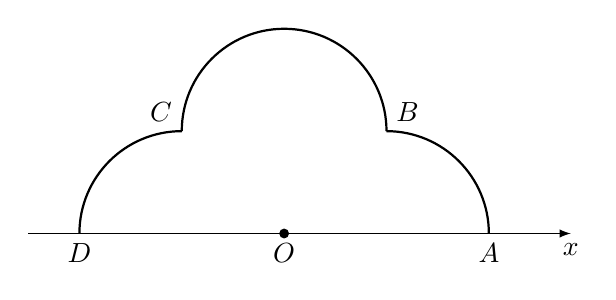
\begin{tikzpicture}[>=latex, scale=1.3]
  % 极轴
  \draw[->] (-2.5,0) -- (2.8,0) node[below] {$x$};
  
  % 原点 O
  \filldraw (0,0) circle (1.2pt) node[below] {$O$};

  % 点 D(-2, 0) 与 点 A(2, 0)
  \coordinate (D) at (-2,0);
  \coordinate (A) at (2,0);
  \node[below] at (D) {$D$};
  \node[below] at (A) {$A$};

  % 弧 AB: 圆心 (1, 0), 半径 1, 极角从 0 到 90 度 (相对于圆心: (2,0) 到 (1,1))
  % 圆心在 (1, 0), 半径 1: (1,0) + (cos t, sin t), t 从 0 到 90 度
  \draw[thick] (1,0) ++(0:1) arc (0:90:1);
  \coordinate (B) at (1,1);
  \node[above right] at (B) {$B$};

  % 弧 BC: 圆心 (0, 1), 半径 1: (0,1) + (cos t, sin t), 从 B(1, 1) 即 t=0 到 (0, 2) 即 t=90 到 C(-1, 1) 即 t=180
  \draw[thick] (0,1) ++(0:1) arc (0:180:1);
  \coordinate (C) at (-1,1);
  \node[above left] at (C) {$C$};

  % 弧 CD: 圆心 (-1, 0), 半径 1: 从 C(-1, 1) 即相对于圆心 (-1, 0) 为 90 度到 180 度即 (-2, 0)
  \draw[thick] (-1,0) ++(90:1) arc (90:180:1);
\end{tikzpicture}\end{center}
\nopagebreak[4]
(1) 分别写出 $M_1, M_2, M_3$ 的极坐标方程;  
(2) 曲线 $M$ 由 $M_1, M_2, M_3$ 构成, 若点 $P$ 在 $M$ 上, 且 $|OP| = \sqrt{3}$, 求 $P$ 的极坐标.

\Needspace{4\baselineskip}
\textbf{解析}

以极点 $O$ 为原点，极轴为 $x$ 轴正半轴建立平面直角坐标系。

\textbf{(1) 解析}
\begin{itemize}
\item 对于弧 $\overset{\frown}{AB}$：
\end{itemize}
  圆心极坐标为 $(1, 0)$，对应直角坐标为 $(1, 0)$。
  由圆经过原点 $O(0, 0)$ 与点 $A(2, 0)$，圆的半径为 1，直角坐标方程为 $(x - 1)^2 + y^2 = 1$，展开得 $x^2 + y^2 - 2x = 0$。
  化为极坐标方程为 $\rho^2 - 2\rho\cos\theta = 0 \implies \rho = 2\cos\theta$。
  点 $A(2, 0)$ 对应 $\theta = 0$，点 $B\left(\sqrt{2}, \dfrac{\pi}{4}\right)$ 对应 $\theta = \dfrac{\pi}{4}$。
\Needspace{5\baselineskip}
  故曲线 $M_1$ 的极坐标方程为：
\nopagebreak[4]
\[M_1: \rho = 2\cos\theta \quad \left(0 \leqslant \theta \leqslant \frac{\pi}{4}\right).\]
\begin{itemize}
\item 对于弧 $\overset{\frown}{BC}$：
\end{itemize}
  圆心极坐标为 $\left(1, \dfrac{\pi}{2}\right)$，对应直角坐标为 $(0, 1)$。
  圆的半径为 1，直角坐标方程为 $x^2 + (y - 1)^2 = 1$，展开得 $x^2 + y^2 - 2y = 0$。
  化为极坐标方程为 $\rho^2 - 2\rho\sin\theta = 0 \implies \rho = 2\sin\theta$。
  点 $B\left(\sqrt{2}, \dfrac{\pi}{4}\right)$ 对应 $\theta = \dfrac{\pi}{4}$，点 $C\left(\sqrt{2}, \dfrac{3\pi}{4}\right)$ 对应 $\theta = \dfrac{3\pi}{4}$。
\Needspace{5\baselineskip}
  故曲线 $M_2$ 的极坐标方程为：
\nopagebreak[4]
\[M_2: \rho = 2\sin\theta \quad \left(\frac{\pi}{4} \leqslant \theta \leqslant \frac{3\pi}{4}\right).\]
\begin{itemize}
\item 对于弧 $\overset{\frown}{CD}$：
\end{itemize}
  圆心极坐标为 $(1, \pi)$，对应直角坐标为 $(-1, 0)$。
  圆的半径为 1，直角坐标方程为 $(x + 1)^2 + y^2 = 1$，展开得 $x^2 + y^2 + 2x = 0$。
  化为极坐标方程为 $\rho^2 + 2\rho\cos\theta = 0 \implies \rho = -2\cos\theta$。
  点 $C\left(\sqrt{2}, \dfrac{3\pi}{4}\right)$ 对应 $\theta = \dfrac{3\pi}{4}$，点 $D(2, \pi)$ 对应 $\theta = \pi$。
\Needspace{5\baselineskip}
  故曲线 $M_3$ 的极坐标方程为：
\nopagebreak[4]
\[M_3: \rho = -2\cos\theta \quad \left(\frac{3\pi}{4} \leqslant \theta \leqslant \pi\right).\]

\textbf{(2) 解析}
设点 $P$ 的极坐标为 $(\rho, \theta)$，由 $|OP| = \sqrt{3}$ 知 $\rho = \sqrt{3}$。
\begin{itemize}
\item 若点 $P$ 在 $M_1$ 上：
\end{itemize}
  由 $\rho = 2\cos\theta = \sqrt{3}$ 得 $\cos\theta = \dfrac{\sqrt{3}}{2}$。
  因为 $0 \leqslant \theta \leqslant \dfrac{\pi}{4}$，解得 $\theta = \dfrac{\pi}{6}$。
  此时点 $P$ 的极坐标为 $\left(\sqrt{3}, \dfrac{\pi}{6}\right)$。
\begin{itemize}
\item 若点 $P$ 在 $M_2$ 上：
\end{itemize}
  由 $\rho = 2\sin\theta = \sqrt{3}$ 得 $\sin\theta = \dfrac{\sqrt{3}}{2}$。
  因为 $\dfrac{\pi}{4} \leqslant \theta \leqslant \dfrac{3\pi}{4}$，解得 $\theta = \dfrac{\pi}{3}$ 或 $\theta = \dfrac{2\pi}{3}$。
  此时点 $P$ 的极坐标为 $\left(\sqrt{3}, \dfrac{\pi}{3}\right)$ 或 $\left(\sqrt{3}, \dfrac{2\pi}{3}\right)$。
\begin{itemize}
\item 若点 $P$ 在 $M_3$ 上：
\end{itemize}
  由 $\rho = -2\cos\theta = \sqrt{3}$ 得 $\cos\theta = -\dfrac{\sqrt{3}}{2}$。
  因为 $\dfrac{3\pi}{4} \leqslant \theta \leqslant \pi$，解得 $\theta = \dfrac{5\pi}{6}$。
  此时点 $P$ 的极坐标为 $\left(\sqrt{3}, \dfrac{5\pi}{6}\right)$。
综上，点 $P$ 的极坐标为 $\left(\sqrt{3}, \dfrac{\pi}{6}\right)$，$\left(\sqrt{3}, \dfrac{\pi}{3}\right)$，$\left(\sqrt{3}, \dfrac{2\pi}{3}\right)$，$\left(\sqrt{3}, \dfrac{5\pi}{6}\right)$。

\gkanswer{答案（1）：$M_1: \rho = 2\cos\theta\ (0 \leqslant \theta \leqslant \dfrac{\pi}{4})$，$M_2: \rho = 2\sin\theta\ (\dfrac{\pi}{4} \leqslant \theta \leqslant \dfrac{3\pi}{4})$，$M_3: \rho = -2\cos\theta\ (\dfrac{3\pi}{4} \leqslant \theta \leqslant \pi)$}

\gkanswer{答案（2）：$\left(\sqrt{3}, \dfrac{\pi}{6}\right)$，$\left(\sqrt{3}, \dfrac{\pi}{3}\right)$，$\left(\sqrt{3}, \dfrac{2\pi}{3}\right)$，$\left(\sqrt{3}, \dfrac{5\pi}{6}\right)$}

\end{answer}
\begin{answer}
\gksolhead{23}{}

\textbf{题目}[选修 4—5：不等式选讲]（10 分）：

设 $x, y, z \in \mathbb{R}$, 且 $x + y + z = 1$.

(1) 求 $(x - 1)^2 + (y + 1)^2 + (z + 1)^2$ 的最小值;  
(2) 若 $(x - 2)^2 + (y - 1)^2 + (z - a)^2 \geqslant \dfrac{1}{3}$ 成立, 证明: $a \leqslant -3$ 或 $a \geqslant -1$.

\Needspace{4\baselineskip}
\textbf{解析}

已知 $x, y, z \in \mathbb{R}$，且 $x + y + z = 1$。

\textbf{(1) 解析}
\Needspace{5\baselineskip}
由柯西不等式：
\nopagebreak[4]
\[[(x - 1)^2 + (y + 1)^2 + (z + 1)^2](1^2 + 1^2 + 1^2) \geqslant [(x - 1) + (y + 1) + (z + 1)]^2.\]
\Needspace{5\baselineskip}
因为 $x + y + z = 1$，所以：
\nopagebreak[4]
\[(x - 1) + (y + 1) + (z + 1) = x + y + z + 1 = 1 + 1 = 2.\]
\Needspace{5\baselineskip}
代入得：
\nopagebreak[4]
\[3[(x - 1)^2 + (y + 1)^2 + (z + 1)^2] \geqslant 2^2 = 4,\]
\Needspace{5\baselineskip}
从而：
\nopagebreak[4]
\[(x - 1)^2 + (y + 1)^2 + (z + 1)^2 \geqslant \frac{4}{3}.\]
当且仅当 $x - 1 = y + 1 = z + 1$，即 $x = \dfrac{5}{3}, y = -\dfrac{1}{3}, z = -\dfrac{1}{3}$ 时等号成立。
因此 $(x - 1)^2 + (y + 1)^2 + (z + 1)^2$ 的最小值为 $\dfrac{4}{3}$。

\textbf{(2) 解析}
\Needspace{5\baselineskip}
由柯西不等式：
\nopagebreak[4]
\[[(x - 2)^2 + (y - 1)^2 + (z - a)^2](1^2 + 1^2 + 1^2) \geqslant [(x - 2) + (y - 1) + (z - a)]^2.\]
\Needspace{5\baselineskip}
因为 $x + y + z = 1$，所以：
\nopagebreak[4]
\[(x - 2) + (y - 1) + (z - a) = (x + y + z) - (3 + a) = 1 - 3 - a = -(a + 2).\]
\Needspace{5\baselineskip}
代入得：
\nopagebreak[4]
\[3[(x - 2)^2 + (y - 1)^2 + (z - a)^2] \geqslant (a + 2)^2,\]
\Needspace{5\baselineskip}
即：
\nopagebreak[4]
\[(x - 2)^2 + (y - 1)^2 + (z - a)^2 \geqslant \frac{(a + 2)^2}{3}.\]
当且仅当 $x - 2 = y - 1 = z - a$ 时取等号。
因此 $(x - 2)^2 + (y - 1)^2 + (z - a)^2$ 的最小值为 $\dfrac{(a + 2)^2}{3}$。
要使不等式 $(x - 2)^2 + (y - 1)^2 + (z - a)^2 \geqslant \dfrac{1}{3}$ 恒成立，
\Needspace{5\baselineskip}
必须且只需其最小值不小于 $\dfrac{1}{3}$，即：
\nopagebreak[4]
\[\frac{(a + 2)^2}{3} \geqslant \frac{1}{3} \implies (a + 2)^2 \geqslant 1 \implies |a + 2| \geqslant 1.\]
\Needspace{5\baselineskip}
解此绝对值不等式得：
\nopagebreak[4]
\[a + 2 \leqslant -1 \quad \text{\text{或}} \quad a + 2 \geqslant 1 \implies a \leqslant -3 \quad \text{\text{或}} \quad a \geqslant -1.\]
命题得证。

\gkanswer{答案（1）：$\dfrac{4}{3}$}

\gkanswer{答案（2）：证明见解析}

\end{answer}